\section{Anexo técnico}

\subsection{Descripción de la respuesta}

\begin{table}[!htbp]
    \centering
    \caption{Descripción de la demanda a 24 horas (MW), periodo de desarrollo 2015--2018.}
    \small
    \label{tab:respuesta}
    \begin{tabular}{lrrrrrr}
\toprule
País & $n$ & Media & Desv. est. & Mínimo & Mediana & Máximo \\
\midrule
DE & 35\,040 & 55\,834 & 10\,032 & 31\,307 & 55\,471 & 77\,549 \\
ES & 35\,023 & 28\,702 & 4\,575 & 18\,041 & 28\,905 & 41\,015 \\
FR & 35\,016 & 54\,069 & 11\,732 & 30\,426 & 52\,383 & 94\,492 \\
\bottomrule
\end{tabular}
    \\ \textit{\scriptsize{Calculada solo con respuestas observadas del periodo de desarrollo (2015--2018).}}
\end{table}

\begin{figure}[!htbp]
    \centering
        \caption{Perfil medio de la demanda a 24 horas por hora local, día de la semana (L = lunes) y mes del instante objetivo, relativo a la media de cada país (adimensional). Periodo de desarrollo (2015--2018).\label{img:descriptiva}}
        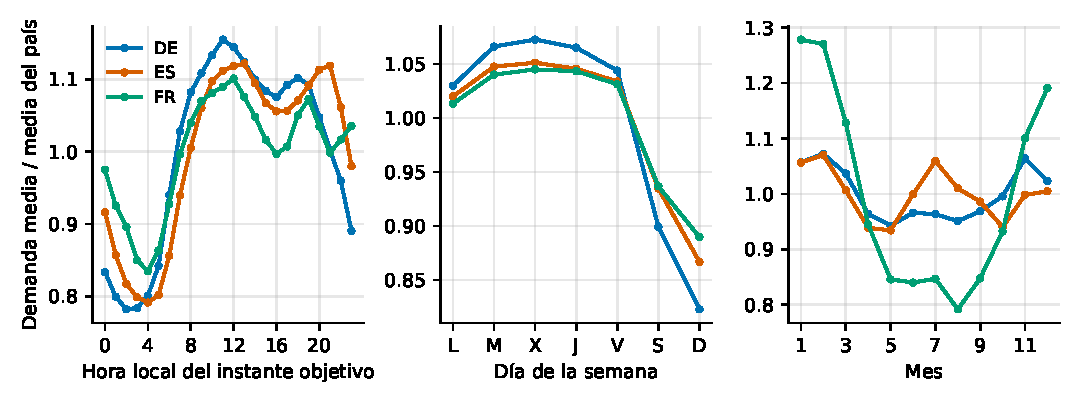
\includegraphics[width=0.95\textwidth]{img/fig_descriptiva.pdf}
\end{figure}

\subsection{Resultados completos de validación}

\begin{table}[!htbp]
    \centering
        \caption{MAE y RMSE (MW) y NMAE por procedimiento, ventana y país; NMAE macro en la última columna.\label{tab:detalle}}
        \resizebox{\textwidth}{!}{\begin{tabular}{llrrrrrrrrrr}
\toprule
 & & \multicolumn{3}{c}{DE} & \multicolumn{3}{c}{ES} & \multicolumn{3}{c}{FR} & Macro \\
\cmidrule(lr){3-5}\cmidrule(lr){6-8}\cmidrule(lr){9-11}
Procedimiento & Ventana & MAE & RMSE & NMAE & MAE & RMSE & NMAE & MAE & RMSE & NMAE & NMAE \\
\midrule
Persistencia & W1 & 4\,492 & 7\,018 & 0{,}0820 & 1\,790 & 2\,760 & 0{,}0630 & 3\,091 & 4\,592 & 0{,}0580 & 0{,}0677 \\
 & W2 & 4\,550 & 7\,007 & 0{,}0826 & 1\,842 & 2\,781 & 0{,}0647 & 3\,023 & 4\,443 & 0{,}0561 & 0{,}0678 \\
 & W3 & 4\,616 & 7\,026 & 0{,}0832 & 1\,824 & 2\,829 & 0{,}0638 & 3\,122 & 4\,575 & 0{,}0579 & 0{,}0683 \\
\midrule
Estacional semanal & W1 & 2\,208 & 4\,006 & 0{,}0403 & 1\,285 & 2\,014 & 0{,}0453 & 3\,458 & 4\,974 & 0{,}0648 & 0{,}0501 \\
 & W2 & 2\,441 & 4\,413 & 0{,}0443 & 1\,458 & 2\,140 & 0{,}0512 & 3\,606 & 5\,161 & 0{,}0669 & 0{,}0542 \\
 & W3 & 2\,557 & 4\,368 & 0{,}0461 & 1\,347 & 2\,111 & 0{,}0471 & 4\,185 & 6\,058 & 0{,}0776 & 0{,}0569 \\
\midrule
M1: Ridge & W1 & 2\,240 & 3\,318 & 0{,}0409 & 1\,157 & 1\,627 & 0{,}0407 & 2\,317 & 3\,204 & 0{,}0434 & 0{,}0417 \\
 & W2 & 2\,325 & 3\,477 & 0{,}0422 & 1\,256 & 1\,752 & 0{,}0441 & 2\,259 & 3\,100 & 0{,}0419 & 0{,}0428 \\
 & W3 & 2\,374 & 3\,458 & 0{,}0428 & 1\,233 & 1\,702 & 0{,}0431 & 2\,489 & 3\,477 & 0{,}0461 & 0{,}0440 \\
\midrule
M2: Árbol podado & W1 & 1\,795 & 3\,158 & 0{,}0328 & 998 & 1\,643 & 0{,}0351 & 2\,326 & 3\,473 & 0{,}0436 & 0{,}0372 \\
 & W2 & 1\,953 & 3\,484 & 0{,}0354 & 960 & 1\,563 & 0{,}0338 & 2\,138 & 3\,225 & 0{,}0397 & 0{,}0363 \\
 & W3 & 1\,819 & 3\,181 & 0{,}0328 & 814 & 1\,404 & 0{,}0285 & 2\,318 & 3\,516 & 0{,}0430 & 0{,}0347 \\
\midrule
M3: Random Forest (dummies) & W1 & 1\,430 & 2\,464 & 0{,}0261 & 755 & 1\,201 & 0{,}0266 & 1\,798 & 2\,700 & 0{,}0337 & 0{,}0288 \\
 & W2 & 1\,537 & 2\,598 & 0{,}0279 & 750 & 1\,214 & 0{,}0264 & 1\,700 & 2\,487 & 0{,}0316 & 0{,}0286 \\
 & W3 & 1\,461 & 2\,395 & 0{,}0263 & 627 & 1\,090 & 0{,}0219 & 1\,805 & 2\,704 & 0{,}0335 & 0{,}0272 \\
\bottomrule
\end{tabular}}
\end{table}

\subsection{Búsqueda de hiperparámetros}

\begin{table}[!htbp]
    \centering
        \caption{Ridge: NMAE macro medio y desviación estándar entre ventanas por valor de $\alpha$ (ordenado por NMAE).\label{tab:ridge}}
        \small
        \begin{tabular}{rrr@{\hspace{1cm}}rrr}
\toprule
$\alpha$ & Media & Desv. est. & $\alpha$ & Media & Desv. est. \\
\midrule
316{,}23 & 0{,}04282 & 0{,}00117 & $3{,}2\times10^{-2}$ & 0{,}04298 & 0{,}00114 \\
100{,}00 & 0{,}04283 & 0{,}00124 & $1{,}0\times10^{-2}$ & 0{,}04298 & 0{,}00114 \\
31{,}62 & 0{,}04291 & 0{,}00120 & $3{,}2\times10^{-3}$ & 0{,}04298 & 0{,}00114 \\
10{,}00 & 0{,}04296 & 0{,}00116 & $1{,}0\times10^{-3}$ & 0{,}04298 & 0{,}00114 \\
3{,}16 & 0{,}04297 & 0{,}00115 & 1\,000 & 0{,}04341 & 0{,}00069 \\
1{,}00 & 0{,}04298 & 0{,}00115 & 3\,162 & 0{,}04653 & 0{,}00195 \\
0{,}32 & 0{,}04298 & 0{,}00115 & 10\,000 & 0{,}05733 & 0{,}00763 \\
0{,}10 & 0{,}04298 & 0{,}00114 &  &  &  \\
\bottomrule
\end{tabular}
    \\ Entre $\alpha=0{,}001$ y $316$ el NMAE es prácticamente constante: el resultado es insensible al valor exacto.
\end{table}

\textbf{Random Forest.} Se evaluaron 18 configuraciones (200 árboles; profundidad máxima ninguna, 15 o 25; mínimo de observaciones por hoja 2, 5 o 10; fracción de predictores 0,7 o 1,0). La configuración seleccionada obtuvo 0,02821 (desviación estándar 0,00085; mínimo 0,02724 en W3 y máximo 0,02880 en W1). La siguiente mejor (profundidad máxima 25) difiere en solo 0,00001, por lo que ambas son prácticamente equivalentes. La tabla \ref{tab:rf_busqueda} entrega las 18 configuraciones.

\begin{table}[!htbp]
    \centering
        \caption{Random Forest: NMAE macro por configuración (promedio, desviación estándar, mínimo y máximo entre ventanas), ordenado por promedio. Todas con 200 árboles.\label{tab:rf_busqueda}}
        \small
        \begin{tabular}{rrrrrrr}
\toprule
\texttt{max\_depth} & \texttt{min\_samples\_leaf} & \texttt{max\_features} & Media & Desv. est. & Mínimo & Máximo \\
\midrule
ninguna & 2 & 0{,}7 & 0{,}02821 & 0{,}00085 & 0{,}02724 & 0{,}02880 \\
25 & 2 & 0{,}7 & 0{,}02822 & 0{,}00084 & 0{,}02726 & 0{,}02878 \\
15 & 2 & 0{,}7 & 0{,}02847 & 0{,}00072 & 0{,}02765 & 0{,}02890 \\
25 & 5 & 0{,}7 & 0{,}02853 & 0{,}00084 & 0{,}02756 & 0{,}02910 \\
ninguna & 5 & 0{,}7 & 0{,}02856 & 0{,}00084 & 0{,}02760 & 0{,}02912 \\
15 & 5 & 0{,}7 & 0{,}02869 & 0{,}00079 & 0{,}02778 & 0{,}02916 \\
ninguna & 2 & 1{,}0 & 0{,}02894 & 0{,}00100 & 0{,}02779 & 0{,}02962 \\
25 & 2 & 1{,}0 & 0{,}02894 & 0{,}00101 & 0{,}02779 & 0{,}02964 \\
15 & 2 & 1{,}0 & 0{,}02918 & 0{,}00088 & 0{,}02816 & 0{,}02969 \\
ninguna & 5 & 1{,}0 & 0{,}02919 & 0{,}00096 & 0{,}02809 & 0{,}02983 \\
25 & 5 & 1{,}0 & 0{,}02920 & 0{,}00096 & 0{,}02809 & 0{,}02984 \\
25 & 10 & 0{,}7 & 0{,}02920 & 0{,}00089 & 0{,}02818 & 0{,}02983 \\
ninguna & 10 & 0{,}7 & 0{,}02921 & 0{,}00089 & 0{,}02819 & 0{,}02983 \\
15 & 10 & 0{,}7 & 0{,}02927 & 0{,}00085 & 0{,}02829 & 0{,}02985 \\
15 & 5 & 1{,}0 & 0{,}02933 & 0{,}00088 & 0{,}02831 & 0{,}02986 \\
ninguna & 10 & 1{,}0 & 0{,}02973 & 0{,}00102 & 0{,}02856 & 0{,}03042 \\
25 & 10 & 1{,}0 & 0{,}02973 & 0{,}00102 & 0{,}02856 & 0{,}03042 \\
15 & 10 & 1{,}0 & 0{,}02979 & 0{,}00098 & 0{,}02866 & 0{,}03043 \\
\bottomrule
\end{tabular}
\end{table}

\subsection{Complejidad, costo e importancia del modelo final}

\begin{table}[!htbp]
    \centering
        \caption{Complejidad de los modelos finales ajustados con el periodo de desarrollo completo (2015--2018).\label{tab:complejidad}}
        \small
        \begin{tabular}{lrrrrr}
\toprule
Modelo final & Árboles & Profundidad media & Profundidad máxima & Nodos & Hojas \\
\midrule
Random Forest (cíclico) & 200 & 35{,}2 & 44 & 11\,412\,818 & 5\,706\,509 \\
Árbol podado & 1 & 26{,}0 & 26 & 8\,521 & 4\,261 \\
\bottomrule
\end{tabular}
\end{table}

\begin{table}[!htbp]
    \centering
        \caption{Tiempo de ajuste final de cada procedimiento con el periodo de desarrollo completo (2015--2018).\label{tab:tiempos}}
        \small
        \begin{tabular}{lr}
\toprule
Procedimiento & Ajuste final (s) \\
\midrule
M1: Ridge & 0{,}1 \\
M2: Árbol podado & 70{,}3 \\
M3: Random Forest (dummies) & 142{,}1 \\
M3$^\ast$: Random Forest (cíclico) & 8{,}5 \\
\bottomrule
\end{tabular}
\end{table}

\begin{table}[!htbp]
    \centering
        \caption{Importancia basada en impureza del Random Forest cíclico final (ajustado con 2015--2018), agrupada por predictor original (seno y coseno de una variable se suman).\label{tab:importancia}}
        \small
        \begin{tabular}{lr@{\hspace{1.2cm}}lr}
\toprule
Predictor & Importancia & Predictor & Importancia \\
\midrule
\texttt{lag\_168h} & 0{,}6468 & \texttt{rolling\_mean\_168h} & 0{,}0089 \\
\texttt{demand\_mw} & 0{,}2474 & \texttt{rolling\_mean\_24h} & 0{,}0083 \\
\texttt{lag\_48h} & 0{,}0499 & \texttt{target\_hour} & 0{,}0035 \\
\texttt{target\_day} & 0{,}0161 & \texttt{target\_month} & 0{,}0029 \\
\texttt{lag\_72h} & 0{,}0150 & \texttt{country} & 0{,}0012 \\
\bottomrule
\end{tabular}
\end{table}

\subsection{Incertidumbre y diagnóstico}

\begin{figure}[!htbp]
    \centering
        \caption{Distribución bootstrap de la diferencia de NMAE macro entre el Random Forest cíclico y la referencia estacional semanal (2\,000 réplicas por bloques semanales). Las líneas discontinuas marcan el intervalo de 95\,\%.\label{img:bootstrap}}
        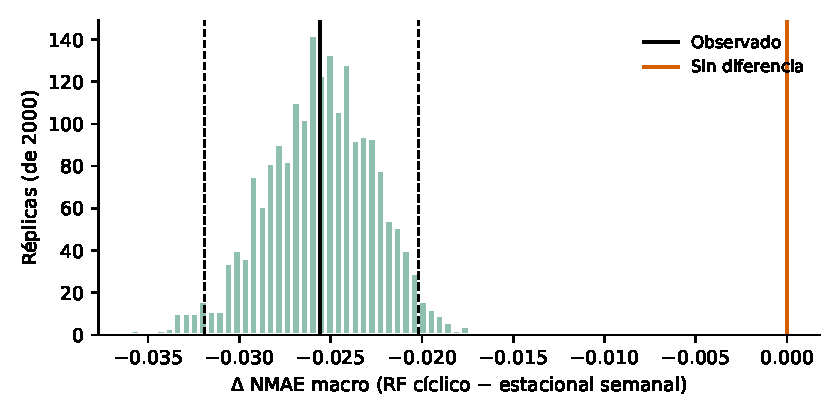
\includegraphics[width=0.62\textwidth]{img/fig_bootstrap.pdf}
\end{figure}

\begin{table}[!htbp]
    \centering
        \caption{Los tres días objetivo con mayor MAE diario del Random Forest cíclico en 2019, por país.\label{tab:peores}}
        \footnotesize
        \begin{tabular}{llp{4.2cm}rrr}
\toprule
País & Fecha objetivo & Feriado nacional & MAE RF (MW) & MAE estac. (MW) & Sesgo RF (MW) \\
\midrule
DE & 03-10-2019 & Día de la Unidad Alemana & 11\,240 & 12\,150 & 11\,240 \\
 & 01-05-2019 & Día del Trabajo & 10\,916 & 12\,761 & 10\,916 \\
 & 19-04-2019 & Viernes Santo & 10\,377 & 15\,033 & 10\,377 \\
\midrule
ES & 25-12-2019 & Navidad & 7\,168 & 10\,347 & 7\,168 \\
 & 01-05-2019 & Día del Trabajo & 4\,430 & 5\,954 & 4\,430 \\
 & 06-12-2019 & Día de la Constitución & 3\,712 & 2\,951 & 3\,633 \\
\midrule
FR & 22-04-2019 & Lunes de Pascua & 8\,962 & 15\,827 & 8\,962 \\
 & 01-05-2019 & Día del Trabajo & 8\,095 & 6\,685 & 8\,095 \\
 & 11-11-2019 & Armisticio & 6\,730 & 3\,645 & 6\,704 \\
\bottomrule
\end{tabular}
    \\ Sesgo = predicción menos observado (positivo: sobreestimación). Los nombres de los feriados provienen del calendario oficial, no de los datos.
\end{table}

\subsection{Resultados completos de la evaluación en 2019}

\begin{table}[!htbp]
    \centering
        \caption{MAE y RMSE (MW) y NMAE por procedimiento y país en la reserva 2019; NMAE macro en la última columna.\label{tab:test_detalle}}
        \resizebox{\textwidth}{!}{\begin{tabular}{lrrrrrrrrrr}
\toprule
 & \multicolumn{3}{c}{DE} & \multicolumn{3}{c}{ES} & \multicolumn{3}{c}{FR} & Macro \\
\cmidrule(lr){2-4}\cmidrule(lr){5-7}\cmidrule(lr){8-10}
Procedimiento & MAE & RMSE & NMAE & MAE & RMSE & NMAE & MAE & RMSE & NMAE & NMAE \\
\midrule
Persistencia & 4\,563 & 6\,951 & 0{,}0817 & 1\,777 & 2\,707 & 0{,}0619 & 3\,098 & 4\,529 & 0{,}0574 & 0{,}0670 \\
\midrule
Estacional semanal & 2\,559 & 4\,469 & 0{,}0458 & 1\,255 & 2\,002 & 0{,}0437 & 3\,337 & 4\,635 & 0{,}0618 & 0{,}0505 \\
\midrule
M1: Ridge & 2\,336 & 3\,462 & 0{,}0418 & 1\,220 & 1\,672 & 0{,}0425 & 2\,084 & 2\,836 & 0{,}0386 & 0{,}0410 \\
\midrule
M2: Árbol podado & 1\,780 & 3\,145 & 0{,}0319 & 785 & 1\,293 & 0{,}0273 & 2\,189 & 3\,317 & 0{,}0406 & 0{,}0333 \\
\midrule
M3: Random Forest (dummies) & 1\,438 & 2\,386 & 0{,}0257 & 611 & 1\,047 & 0{,}0213 & 1\,697 & 2\,507 & 0{,}0314 & 0{,}0262 \\
\midrule
M3$^\ast$: Random Forest (cíclico) & 1\,355 & 2\,227 & 0{,}0243 & 583 & 1\,015 & 0{,}0203 & 1\,626 & 2\,403 & 0{,}0301 & 0{,}0249 \\
\bottomrule
\end{tabular}}
\end{table}

\subsection{Correlación entre predictores}

\begin{table}[!htbp]
    \centering
        \caption{Correlación de Pearson entre los predictores numéricos y la respuesta en el entrenamiento final (2015--2018), calculada dentro de cada país y promediada entre los tres.\label{tab:correlacion}}
        \footnotesize
        \resizebox{\textwidth}{!}{\begin{tabular}{lrrrrrr}
\toprule
 & \texttt{demand\_mw} & \texttt{lag\_48h} & \texttt{lag\_72h} & \texttt{lag\_168h} & \texttt{rolling\_mean\_24h} & \texttt{rolling\_mean\_168h} \\
\midrule
\texttt{lag\_48h} & 0{,}83 &  &  &  &  &  \\
\texttt{lag\_72h} & 0{,}67 & 0{,}83 &  &  &  &  \\
\texttt{lag\_168h} & 0{,}78 & 0{,}64 & 0{,}61 &  &  &  \\
\texttt{rolling\_mean\_24h} & 0{,}67 & 0{,}66 & 0{,}41 & 0{,}37 &  &  \\
\texttt{rolling\_mean\_168h} & 0{,}50 & 0{,}52 & 0{,}53 & 0{,}52 & 0{,}69 &  \\
\texttt{target\_demand\_mw} & 0{,}83 & 0{,}67 & 0{,}62 & 0{,}91 & 0{,}43 & 0{,}48 \\
\bottomrule
\end{tabular}}
    \\ La última fila es la correlación con la respuesta \texttt{target\_demand\_mw}.
\end{table}

\subsection{Datos ausentes}

\begin{table}[!htbp]
    \centering
        \caption{Bloques de horas consecutivas sin demanda observada, por país (2015--2019).\label{tab:ausentes_bloques}}
        \small
        \begin{tabular}{llrr}
\toprule
País & Fecha de inicio (UTC) & Hora & Horas consecutivas \\
\midrule
DE & sin ausentes & -- & 0 \\
\midrule
ES & 01-01-2015 & 00:00 & 1 \\
 & 02-01-2015 & 06:00 & 3 \\
 & 02-01-2015 & 11:00 & 8 \\
 & 01-05-2015 & 10:00 & 6 \\
\midrule
FR & 01-01-2015 & 00:00 & 1 \\
 & 05-02-2017 & 19:00 & 13 \\
 & 12-08-2018 & 07:00 & 5 \\
 & 04-10-2018 & 01:00 & 3 \\
 & 14-12-2018 & 04:00 & 3 \\
 & 25-07-2019 & 00:00 & 5 \\
\bottomrule
\end{tabular}
\end{table}

\begin{table}[!htbp]
    \centering
        \caption{NMAE de cada país con sus casos completos (propio) y restringido a las fechas en que los tres países tienen caso completo (común).\label{tab:ausentes_efecto}}
        \footnotesize
        \resizebox{\textwidth}{!}{\begin{tabular}{llrrrrrrrr}
\toprule
 & & \multicolumn{2}{c}{$n$} & \multicolumn{2}{c}{Estacional} & \multicolumn{2}{c}{Ridge} & \multicolumn{2}{c}{RF cíclico} \\
\cmidrule(lr){3-4}\cmidrule(lr){5-6}\cmidrule(lr){7-8}\cmidrule(lr){9-10}
Periodo & País & Propio & Común & Propio & Común & Propio & Común & Propio & Común \\
\midrule
W1 & DE & 8\,784 & 8\,784 & 0{,}0403 & 0{,}0403 & 0{,}0409 & 0{,}0409 & -- & -- \\
 & ES & 8\,784 & 8\,784 & 0{,}0453 & 0{,}0453 & 0{,}0407 & 0{,}0407 & -- & -- \\
 & FR & 8\,784 & 8\,784 & 0{,}0648 & 0{,}0648 & 0{,}0434 & 0{,}0434 & -- & -- \\
 & Macro & 26\,352 & 26\,352 & 0{,}0501 & 0{,}0501 & 0{,}0417 & 0{,}0417 & -- & -- \\
\midrule
W2 & DE & 8\,760 & 8\,567 & 0{,}0443 & 0{,}0447 & 0{,}0422 & 0{,}0424 & -- & -- \\
 & ES & 8\,760 & 8\,567 & 0{,}0512 & 0{,}0518 & 0{,}0441 & 0{,}0442 & -- & -- \\
 & FR & 8\,567 & 8\,567 & 0{,}0669 & 0{,}0669 & 0{,}0419 & 0{,}0419 & -- & -- \\
 & Macro & 26\,087 & 25\,701 & 0{,}0542 & 0{,}0545 & 0{,}0428 & 0{,}0429 & -- & -- \\
\midrule
W3 & DE & 8\,736 & 8\,213 & 0{,}0461 & 0{,}0463 & 0{,}0428 & 0{,}0434 & -- & -- \\
 & ES & 8\,736 & 8\,213 & 0{,}0471 & 0{,}0465 & 0{,}0431 & 0{,}0430 & -- & -- \\
 & FR & 8\,213 & 8\,213 & 0{,}0776 & 0{,}0776 & 0{,}0461 & 0{,}0461 & -- & -- \\
 & Macro & 25\,685 & 24\,639 & 0{,}0569 & 0{,}0568 & 0{,}0440 & 0{,}0442 & -- & -- \\
\midrule
2019 & DE & 8\,736 & 8\,559 & 0{,}0458 & 0{,}0463 & 0{,}0418 & 0{,}0420 & 0{,}0243 & 0{,}0244 \\
 & ES & 8\,736 & 8\,559 & 0{,}0437 & 0{,}0429 & 0{,}0425 & 0{,}0425 & 0{,}0203 & 0{,}0201 \\
 & FR & 8\,559 & 8\,559 & 0{,}0618 & 0{,}0618 & 0{,}0386 & 0{,}0386 & 0{,}0301 & 0{,}0301 \\
 & Macro & 26\,031 & 25\,677 & 0{,}0505 & 0{,}0503 & 0{,}0410 & 0{,}0410 & 0{,}0249 & 0{,}0249 \\
\bottomrule
\end{tabular}}
    \\ Estacional: referencia estacional semanal. $n$ corresponde a las filas de evaluación del país (en Macro, suma de los tres). Para Francia ambos valores coinciden porque sus fechas son un subconjunto de las de los otros países. El Random Forest cíclico solo se evalúa en 2019.
\end{table}

\pend{PENDIENTE: Agregar al anexo los resultados de las sensibilidades por país.}

\subsection{Costo computacional: CPU frente a GPU} \label{sec:gpu}

Se midió el tiempo de reloj de cada sección de los notebooks y de la validación (\texttt{src/timing.py}) en un computador con CPU AMD Ryzen 5 9600X (12 núcleos lógicos) y GPU NVIDIA RTX 5060 (8 GB), en Ubuntu 24.04 (WSL2), y se repitió con la GPU mediante RAPIDS cuML (\texttt{docs/tiempos\_cpu\_gpu.md}). Es una sola ejecución por configuración, sin repeticiones, por lo que las diferencias pequeñas no son concluyentes.

\textbf{Acelerador automático} (\texttt{cuml.accel}, \texttt{analisis.py --gpu}). Los pasos 3 a 6 tardaron 633 s en CPU y 719 s con GPU (0,88 veces la velocidad de la CPU). Ridge sí se ejecutó en la GPU, pero su primer ajuste pagó 13 s de inicialización; el árbol podado y el Random Forest con indicadores casi no cambiaron de tiempo (134 frente a 139 s en W1--W3), lo que sugiere que siguieron en CPU: cuML no tiene árbol con poda, y una explicación plausible, no verificada, para el bosque es que la codificación con indicadores produce una matriz dispersa.

\textbf{Modelos forzados a la GPU} (\texttt{src/benchmark\_gpu.py}, solo W1--W3). Se ajustaron directamente con cuML, con matriz densa en \texttt{float32} (tabla \ref{tab:gpu}). cuML exige una profundidad máxima finita, por lo que se comparó con scikit-learn con la misma profundidad.

\begin{table}[!htbp]
    \centering
        \caption{Ajuste y predicción en W1--W3 (suma de segundos) y NMAE macro medio, CPU (scikit-learn) frente a GPU (cuML), con matriz densa.\label{tab:gpu}}
        \footnotesize
        \begin{tabular}{@{}lrrrrr@{}}
            \toprule
            Modelo & CPU (s) & GPU (s) & Velocidad GPU/CPU & NMAE CPU & NMAE GPU \\
            \midrule
            Ridge & 0,04 & 0,10 & 0,43 & 0,04282 & 0,04282 \\
            RF indicadores, profundidad 16 & 15,5 & 26,4 & 0,59 & 0,02832 & 0,02844 \\
            RF indicadores, profundidad 32 & 18,6 & 59,7 & 0,31 & 0,02820 & 0,02830 \\
            RF cíclico, profundidad 16 & 13,5 & 15,7 & 0,86 & 0,02716 & 0,02724 \\
            RF cíclico, profundidad 32 & 15,6 & 33,5 & 0,47 & 0,02711 & 0,02722 \\
            \midrule
            RF indicadores, sin límite (oficial) & 18,2 & -- & -- & 0,02821 & -- \\
            \bottomrule
        \end{tabular}
    \\ Velocidad GPU/CPU $<1$: la GPU es más lenta. Excluye 10 s de inicialización de la GPU.
\end{table}

La GPU fue más lenta en todos los casos, más aún con árboles profundos y con más columnas (indicadores), y el NMAE cambió menos de 0,5\,\%. Su desventaja se reduce al crecer el entrenamiento (RF cíclico, profundidad 16: 0,52 en W1, 0,88 en W2 y 1,06 en W3), por lo que con muchas más filas podría convenir; con unas 100\,000, no. La ganancia relevante fue otra: el mismo Random Forest oficial con matriz densa tardó 18 s en W1--W3, frente a 134 s con la matriz dispersa del \textit{pipeline}, con igual NMAE (0,02821). Este cambio no se aplicó a los resultados del informe.

